%----------------------------------------------------------------------------------------
%	PACKAGES AND OTHER DOCUMENT CONFIGURATIONS
%----------------------------------------------------------------------------------------

\documentclass[twoside,twocolumn,a4paper]{article}

\usepackage{blindtext} % Package to generate dummy text throughout this template 

\usepackage[T1]{fontenc} % Use 8-bit encoding that has 256 glyphs
\usepackage{lmodern}

\usepackage{graphicx}

\linespread{1.05} % Line spacing - Palatino needs more space between lines
\usepackage{microtype} % Slightly tweak font spacing for aesthetics

\usepackage[spanish]{babel} % Language hyphenation and typographical rules

\usepackage[numbib,notlof,notlot,nottoc]{tocbibind} % Shows bibliography as a section

\usepackage[hmarginratio=1:1,top=32mm,columnsep=20pt]{geometry} % Document margins

\usepackage[hang, small,labelfont=bf,up,textfont=up]{caption} % Custom captions under/above floats in tables or figures

\usepackage{booktabs} % Horizontal rules in tables

\usepackage{enumitem} % Customized lists

\setlist[itemize]{noitemsep} % Make itemize lists more compact

\usepackage{abstract} % Allows abstract customization

\renewcommand{\abstractnamefont}{\normalfont\bfseries} % Set the "Abstract" text to bold

\usepackage{fancyhdr} % Headers and footers
\pagestyle{fancy} % All pages have headers and footers
\fancyhead{} % Blank out the default header
\fancyfoot{} % Blank out the default footer
\fancyhead[C]{Laboratorio 3 $\bullet$ Informe 1 $\bullet$ Grupo 8: Inafuku, Petino, Poggi} % Custom header text
\fancyfoot[C]{\thepage} % Custom footer text

\usepackage{titling} % Customizing the title section

\usepackage{hyperref} % For hyperlinks in the PDF

%----------------------------------------------------------------------------------------
%	TITLE SECTION
%----------------------------------------------------------------------------------------

\setlength{\droptitle}{-4\baselineskip} % Move the title up

\pretitle{\begin{center}\LARGE\bfseries} % Article title formatting
\posttitle{\end{center}} % Article title closing formatting
\title{Medici\'on de la resistencia de una l\'ampara incandescente} % Article title
\author{%
\textsc{Maximiliano Inafuku} \\[1ex] % Your name
\normalsize \href{mailto:maxi-46@hotmail.com}{maxi-46@hotmail.com} % Your email address
\and % Uncomment if 2 authors are required, duplicate these 4 lines if more
\textsc{Ernesto Petino} \\[1ex] % Second author's name
\normalsize \href{mailto:ernesto.atmo@gmail.com}{ernesto.atmo@gmail.com} % Second author's email address
\and % Uncomment if 2 authors are required, duplicate these 4 lines if more
\textsc{Ignacio Poggi} \\[1ex] % Second author's name
\normalsize \href{mailto:ignaciop.3@gmail.com}{ignaciop.3@gmail.com} % Second author's email address
}

\date{Grupo 8 - Laboratorio 3, C\'atedra Bilbao - Departamento de F\'isica, Facultad de Ciencias Exactas y Naturales, Universidad de Buenos Aires \newline \\ \today} % Leave empty to omit a date
\renewcommand{\maketitlehookd}{%
\begin{abstract}
\noindent En este trabajo se arm\'o un circuito electr\'onico simple para medir la resistencia de una l\'ampara incandescente. Se caracterizaron las resistencias internas de la fuente, volt\'imetro y amper\'imetro utilizados en dicho circuito. Se analizaron los datos obtenidos con el programa Origin y se encontr\'o que la correspondiente a la l\'ampara se ve afectada por la temperatura de su filamento y por la del ambiente.
\end{abstract}
}

%----------------------------------------------------------------------------------------

\begin{document}

% Print the title
\maketitle

%----------------------------------------------------------------------------------------
%	ARTICLE CONTENTS
%----------------------------------------------------------------------------------------

\section{Introducci\'on}

La corriente en un conductor viene dada por un campo el\'ectrico $\mathbf{\vec{E}}$ dentro del conductor que ejerce una fuerza $q\mathbf{\vec{E}}$ sobre las cargas libres. Dichas cargas circulan por el conductor conducidas por las fuerzas debidas al campo el\'ectrico. En un metal, las cargas libres al ser negativas, se mueven en direcci\'on opuesta a $\mathbf{\vec{E}}$ que al interactuar con los iones del material utilizado como conductor, producen fuerzas que se oponen a su movimiento.\par
Como el campo el\'ectrico est\'a siempre dirigido desde las regiones de mayor potencial hacia las de menor potencial, y adem\'as consideramos la corriente como un flujo de cargas positivas, las mismas se mueven en la direcci\'on y el sentido en el que el potencial decrece. Por lo tanto, la diferencia de potencial $V$ entre los puntos $a$ y $b$ (mayor y menor potencial, respectivamente) es \cite{eq:potencial}:
\begin{equation}
\label{eq:potencial}
V = V_{a} - V_{b} = E\Delta L
\end{equation}
donde $\Delta L$ es la longitud de un segmento arbitrario por donde circula la corriente $I$.
\par El cociente entre la ca\'ida de potencial en la direcci\'on de la corriente y la intensidad de \'esta \'ultima se denomina \textbf{resistencia} del segmento \cite{eq:ohm1}:
\begin{equation}
\label{eq:ohm1}
R = \frac{V}{I}
\end{equation}
\par Para muchos materiales, la resistencia no depende de la ca\'ida de voltaje ni de la intensidad. Estos materiales se denominan \'ohmicos, y su caracter\'istica a destacar es que la ca\'ida de potencial a trav\'es de un conductor es proporcional a la corriente (relaci\'on lineal).
\par En estos materiales, $R$ permanece aproximadamente constante, en otros casos (materiales no \'ohmicos) puede variar dependiendo de caracter\'isticas f\'isicas intensivas del material o del entorno (como la temperatura, humedad, etc.). Esta relaci\'on se conoce como la \textit{Ley de Ohm} y se escribe normalmente como \cite{eq:ohm2}:
\begin{equation}
\label{eq:ohm2}
V = IR
\end{equation}
\par En este trabajo veremos como var\'ia la resistencia de la l\'ampara incandescente en funci\'on de la intensidad de corriente circulando en el circuito; teniendo en cuenta la temperatura del filamento y la del ambiente.

%------------------------------------------------

\section{Dispositivo experimental}

Los instrumentos de laboratorio utilizados fueron:
\begin{itemize}
\item 
\label{Fuente} Fuente de corriente continua, Hantek PPS-2320A (R\'otulo: FC-04)
\cite{Fuente}
\item 
\label{amp} Mult\'imetro Protek 506, utilizado como amper\'imetro (R\'otulo: 4)
\cite{amp}
\item 
\label{volt} Mult\'imetro UNI-T UT55, utilizado como volt\'imetro (R\'otulo: 2)
\cite{volt}
\item L\'ampara incandescente
\end{itemize}

Para lograr hallar la resistencia de la l\'ampara incandescente fue necesario medir la ca\'ida de potencial y la corriente que circulaba por esta. Para ello se coloc\'o en serie la l\'ampara incandescente y el amper\'imetro y conectados a estos en paralelo el volt\'imetro y la fuente de corriente continua (Figura \ref{fig:dsp_exp}).\par

\begin{figure}
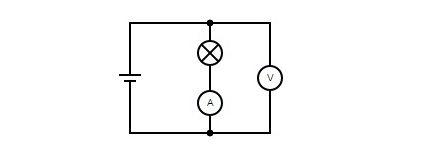
\includegraphics[width=\linewidth]{dispositivo_experimental.jpg}
\caption{Esquema del circuito realizado.}
\label{fig:dsp_exp}
\end{figure}

Se realizaron luego las mediciones, variando la diferencia de potencial de la fuente de corriente continua y tomando los datos de la corriente que pasaba por el amper\'imetro. Debido a que las mediciones se ve\'ian considerablemente afectadas por el ambiente externo (ya que la temperatura afectaba la resistencia, y por ende la corriente) fue necesario aislar de forma parcial a la l\'ampara del medio ambiente. Para ello se coloc\'o una cobertura pl\'astica que cubr\'ia a la misma. Luego, para cada medici\'on de intensidad se esper\'o a que se estabilizara la temperatura de la l\'ampara.

%------------------------------------------------
\section{Resultados y an\'alisis}

Con los datos obtenidos se grafic\'o la diferencial de potencial registrada por el volt\'imetro en funci\'on de la intensidad. Luego se realizaron un ajuste lineal (Figura 2), uno de orden dos con el origen forzado (Figura 3), uno de orden dos con todos los par\'ametros libres (Figura 4) y finalmente uno de orden tres. 


\begin{table}
\caption{Ajustes Realizados}
\centering
\begin{tabular}{llr}
\toprule
\multicolumn{2}{c}{Ajuste polin\'omicos} \\
\cmidrule(r){1-2}
Orden 2 & Orden 3 & Lineal\\
\midrule
John & Doe & $7.5$ \\
Richard & Miles & $2$ \\
\bottomrule
\end{tabular}
\end{table}


%------------------------------------------------

\section{Conclusiones}


%----------------------------------------------------------------------------------------
%	REFERENCE LIST
%----------------------------------------------------------------------------------------

\begin{thebibliography}{99} % Bibliography - this is intentionally simple in this template

\bibitem{eq:potencial} E. M. Purcell, \textit{Electricidad y Magnetismo - Berkeley Physics Course Vol. 2}, Editorial Revert\'e S.A., 2da edici\'on, Barcelona (1988), p\'ag. 124
\bibitem{eq:ohm1} E. M. Purcell, \textit{Electricidad y Magnetismo - Berkeley Physics Course Vol. 2}, Editorial Revert\'e S.A., 2da edici\'on, Barcelona (1988), p\'ag. 124
\bibitem{eq:ohm2} E. M. Purcell, \textit{Electricidad y Magnetismo - Berkeley Physics Course Vol. 2}, Editorial Revert\'e S.A., 2da edici\'on, Barcelona (1988), p\'ag. 123
\bibitem{Fuente}
\bibitem{amp} https://www.scribd.com/doc/222262447/Manual-y-Diagrama-Esquematico-de-Multimetro-Digital-Protek-506
\bibitem{volt} http://www.ageta.hu/pdf/UT51-55.pdf
 
\end{thebibliography}

%----------------------------------------------------------------------------------------

\end{document}